\documentclass[a4paper]{article}

\usepackage[english]{babel}
\usepackage[utf8x]{inputenc}
\usepackage[T1]{fontenc}
\usepackage[a4paper,top=2cm,bottom=2cm,left=3cm,right=3cm,marginparwidth=1.75cm]{geometry}
\usepackage{amsmath}
\usepackage{graphicx}
\usepackage[colorinlistoftodos]{todonotes}
\usepackage[colorlinks=true, allcolors=blue]{hyperref}
\usepackage{float}
\usepackage{enumerate}
\usepackage{subfig}
\usepackage{ctex}
\usepackage{listings}
\usepackage{xcolor}
\usepackage{siunitx}
\usepackage{multirow}
\usepackage{color}
\usepackage{hyperref}

\hypersetup{hypertex=true, colorlinks=true, linkcolor=blue, anchorcolor=blue, citecolor=blue}

\title{计算理论导论 —— 期末复习}
\author{陈志朋}
\date{}
\begin{document}
	\maketitle
	\tableofcontents

\section{总览}

	所有语言的关系如图\ref{F01}。
	\begin{figure}[htb]
		\centering
		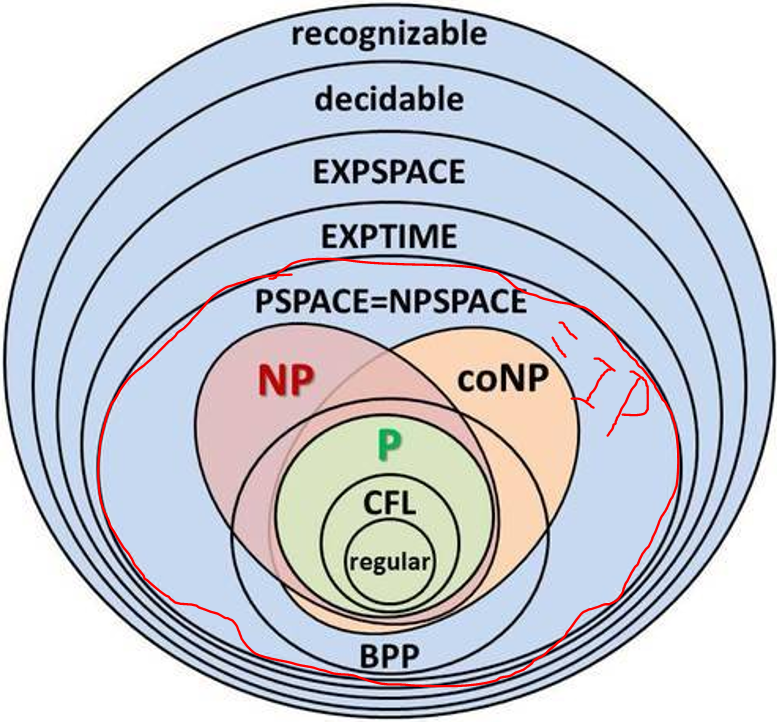
\includegraphics[scale=0.4]{./figure/1.png}
		\caption{Overview}
		\label{F01}
   \end{figure} 

\section{正则语言}

\subsection{有穷自动机}

\subsubsection{有穷自动机的形式定义}

	\colorbox{yellow}{定义2.1} 有穷自动机是一个$5$元组$(Q,\Sigma,\delta, q_0, F)$:
	
	\qquad 1) $Q$是一个有穷集合,叫做\textbf{状态集}。
	
	\qquad 2) $\Sigma$是一个有穷集合,叫做\textbf{字母集}。
	
	\qquad 3) $\delta: Q \times \Sigma \rightarrow Q$是\textbf{转移函数}。
	
	\qquad 4) $q_0 \in Q$是\textbf{起始状态}。
	
	\qquad 5) $F \subseteq Q$是接受状态集。
	
\subsubsection{有穷自动机举例}
	
	\colorbox{pink}{例2.3} 接受语言$L(M)=\{w|w~is~the~empty~string~\varepsilon~or~ends~in~a~0\}$的DFA,示意图 \ref{F020102}

	\begin{figure}[htb]
		\centering
		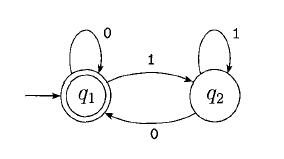
\includegraphics[scale=0.8]{./figure/2.1.2.png}
		\caption{A~DFA~of~language~$M$}
		\label{F020102}
	\end{figure}

\subsubsection{计算的形式定义}

	当一个字符串$w$从有穷自动机的起始状态开始,按照转移函数从一个状态到一个状态,并且机器结束在接受状态,则称\textbf{$M$接受$w$}。如果$A=\{w|M accepts w\}$,则称\textbf{$M$识别语言$A$}。

	\colorbox{yellow}{定义2.7} 如果一个语言被一台\textbf{有穷自动机}识别,则称它是\textbf{正则语言}。

\subsubsection{设计有穷自动机}

	\colorbox{pink}{例2.9} 有穷自动机$E_2$识别含有$001$作为子串的所有字符串组成的正则语言,示意图 \ref{F020104}

	\begin{figure}[htb]
		\centering
		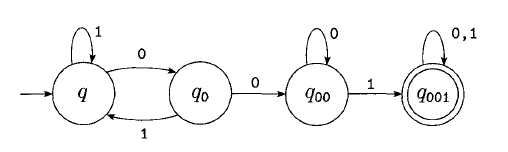
\includegraphics[scale=0.8]{./figure/2.1.4.png}
		\caption{DFA~$E_2$}
		\label{F020104}
	\end{figure}
	
\subsubsection{正则运算}

	\colorbox{yellow}{定义2.10} 设$A$和$B$是两个语言,定义正则运算\textbf{并}、\textbf{连接}和\textbf{星号}如下:
	
	\qquad \textbf{并}: $A \cup B = \{x|x \in A~or~x \in B\}$
	
	\qquad \textbf{连结}: $A \circ B = \{xy|x \in A~and~y \in B\}$
	
	\qquad \textbf{星号}: $A^* = \{x_1 \dot x_k|k \geq 0~and~\forall x_i \in A\}$

	\colorbox{green}{定理2.12} 正则语言类在并运算下封闭。
	
	\textbf{证明思路} 
	\qquad 设$M_1={Q_1,\Sigma,\delta_1,q_1,F_1}$可以识别$A$,设$M_2={Q_2,\Sigma,\delta_2,q_2,F_2}$可以识别$B$。
	\qquad 构造$M={Q_1 \times Q_2,\Sigma,\delta,(q_1, q_2),(F_1 \times Q_2) \cup (F_2 \times Q_1)}$,其中$\delta((r_1,r_2), a)=(\delta_1(r_1,a), \delta_2(r_2, a))$,可以识别$A \cup B$。
	
	\colorbox{green}{定理2.13} 正则语言类在连结运算下封闭。
	
	\textbf{证明思路} \quad 引入非确定性的新技术,即使用非确定型有穷自动机来证明。

\subsection{非确定性}

\subsubsection{非确定型有穷自动机的形式定义}

	\colorbox{yellow}{定义2.17} \textbf{非确定型有穷自动机}是一个$5$元组$(Q, \Sigma, \delta, q_0, F)$,其中
	
	\qquad 1) $Q$是有穷的状态集。
	
	\qquad 2) $\Sigma$是有穷的字母表。

	\qquad 3) $\delta:Q\times \Sigma_{\varepsilon} \rightarrow \mathcal{P}(Q)$是转移函数。
	
	\qquad 4) $q_0 \in Q$是起始状态。
	
	\qquad 5) $F \subseteq Q$是接受状态集。

\subsubsection{NFA与DFA的等价性}

	\colorbox{green}{定理2.19} 每一台非确定型有穷自动机都有一条等价的确定型有穷自动机。
	
	\textbf{证明思路} \quad 把能到达的子集合并,构造新的状态。

	\colorbox{gray}{推论2.20} 一个语言是正则的,当且仅当有一台非确定型的有穷自动机识别它。
	
	\textbf{证明思路} \quad NFA和DFA等价。

\subsubsection{在正则运算下的封闭性}

	\colorbox{green}{定理2.22}  正则语言在并运算下封闭。
	
	\textbf{证明思路} \quad 示意图 \ref{F020203-1}。
	\begin{figure}[htb]
		\centering
		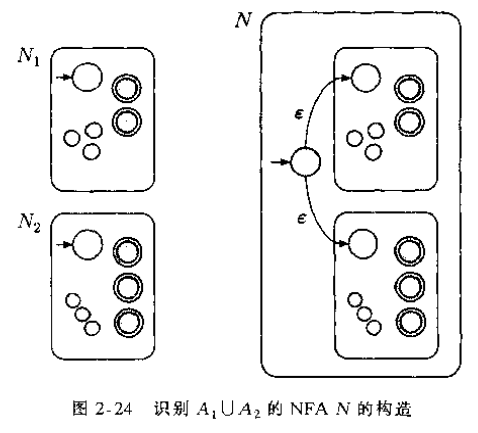
\includegraphics[scale=0.8]{./figure/2.2.3-1.png}
		\caption{NFA~recognizes~$A=A_1 \cup A_2$}
		\label{F020203-1}
	\end{figure}

	\colorbox{green}{定理2.23}  正则语言在连结运算下封闭。
	
	\textbf{证明思路} \quad 示意图 \ref{F020203-2}。
	\begin{figure}[htb]
		\centering
		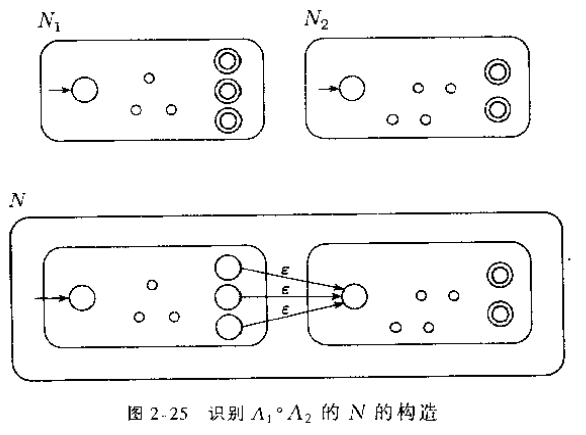
\includegraphics[scale=0.8]{./figure/2.2.3-2.png}
		\caption{NFA~recognizes~$A=A_1 \circ A_2$}
		\label{F020203-2}
	\end{figure}

	\colorbox{green}{定理2.22}  正则语言在星号运算下封闭。
	
	\textbf{证明思路} \quad 示意图 \ref{F020203-3}。

	\begin{figure}[htb]
		\centering
		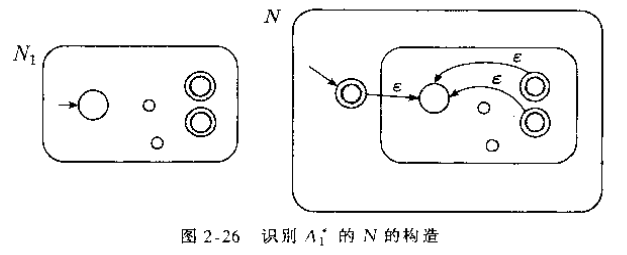
\includegraphics[scale=0.8]{./figure/2.2.3-3.png}
		\caption{NFA~recognizes~$A=A_1^*$}
		\label{F020203-3}
	\end{figure}

\subsection{正则表达式}

\subsubsection{正则表达式的形式定义}

	\colorbox{yellow}{定义2.26} 称$R$是一个正则表达式,如果$R$是:
	
	\qquad 1) $a$,这里的$a$是字母表$\Sigma$中的一个元素。
	
	\qquad 2) $\varepsilon$ 。
	
	\qquad 3) $\emptyset$ 。
	
	\qquad 4) $(R_1 \cup R_2)$,这里的$R_1$和$R_2$是正则表达式。
	
	\qquad 5) $(R_1 \circ R_2)$,这里的$R_1$和$R_2$是正则表达式。
	
	\qquad 6) $(R_1^*)$,这里的$R_1$是正则表达式。

	连接符号和括号可以省略。如果没有括号,优先级从高到低为:星号、连结、并。
	
\subsubsection{与有穷自动机的等价性}

	\colorbox{green}{定理2.28} 一个语言是正则的,当且仅当可以用正则表达式描述它。
	
	\textbf{证明思路} \quad 使用引理2.29和引理2.30。
	
	\colorbox{cyan}{引理2.29} 如果一个语言可以用正则表达式描述,则它是正则的。
	
	\textbf{证明思路} \quad 对于每种正则运算有对应的NFA构造方法。
	
	\colorbox{cyan}{引理2.30} 如果一个语言是正则的,则它可以用正则表达式描述。
	
	\textbf{证明思路} \quad 把DFA转化为GNFA,然后把GNFA转化为正则表达式。
	
	\colorbox{yellow}{定义2.33} \textbf{广义非确定型有穷自动机}$(Q,\Sigma,\delta,q_{start},q_{accept})$是一个$5$元组,其中:
	
	\qquad 1) $Q$是有穷的状态集。

	\qquad 2) $\Sigma$是输入字母表。
	
	\qquad 3) $\delta:(Q-\{q_{accept}\})\times(Q-\{q_{start}\})$。
	
	\qquad 4) $q_{start}$是起始状态。
	
	\qquad 5) $q_{accept}$是接受状态。
	
	如果字符串$w$可写成$w=w_1,w_2 \dots w_k$,这里每一个$w_i \in \Sigma^*$,并且存在状态序列$q_0,q_1,\dots,q_k$,使得:
	
	\qquad 1) $q_0=q_{start}$是起始状态。
	
	\qquad 2) $q_0=q_{accept}$是接受状态。
	
	\qquad 3)对于每一个$i$,$w_i \in L(R_i)$,其中$R_i=\delta(q_{i-1},q_i)$,换句话说,$R$是从$q_{i-1}$到$q_i$的箭头上的表达式。
	
	则称这台GNFA接受字符串$w$。

	\textbf{GNFA的特殊形式}:
	
	\qquad 1) 起始状态有射到其他每一个状态的箭头,但是没有从任何其他状态射入的箭头。
	
	\qquad 2) 有唯一的一个接受状态,并且他有从每一个状态射入的箭头,但是没有射到任何其他状态的箭头。此外,这个接受状态与其实状态不同。
	
	\qquad 3) 除起始状态和接受状态之外,每一个状态到自身和其他每一个状态都有一个箭头。
	
	\textbf{DFA到GNFA的转化}:添加新的起始状态和新的接受状态,从新起始状态到老起始状态有一个$\varepsilon$箭头,从每一个老接受状态到新接受状态有一个$\varepsilon$箭头。对于其他状态,没有边的连一个$\emptyset$的箭头,一条边上有多个的字母的取并集。
	
	\textbf{GNFA到正则表达式的转化}:当状态数$k>2$时,选取一个状态(非起始状态和接受状态),删除这个状态,然后对其他状态的路径进行修改,示意图 \ref{F020302}。
	
	\begin{figure}[htb]
		\centering
		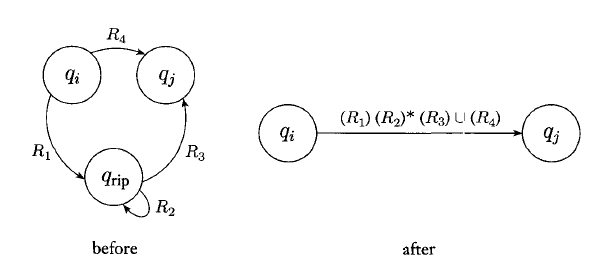
\includegraphics[scale=0.8]{./figure/2.3.2.png}
		\caption{Delete $q_{rip}$}
		\label{F020302}
	\end{figure}

\subsection{非正则语言}

	\colorbox{green}{定理2.37} 泵引理(Pumping Lemma)
	
	设$A$是一个正则语言,则存在一个数$p$(泵长度Pumping Length)使得,如果$s$是$A$中任一长度不小于$p$的字符串,那么$s$可以被分成$3$段,$s=xyz$,满足下述条件:
	
	\qquad 1) 对\textbf{每一个$i \geq 0$},$xyz \in A$
	
	\qquad 2) $|y|>0$
	
	\qquad 2) $|xy| \leq p$

	\textbf{证明思路} \quad 设$M$是识别$A$的DFA,令泵长度(Pumping Length)$p$等于$M$的状态数,起始节点也算一个状态,所以一共经过了$p+1$个状态。根据鸽笼原理一定会经过重复结点,这个重复状态(即$y$)可以进行扩展,也可以把这段删除。
	
	\colorbox{pink}{例2.38} 证明语言$B=\{0^n1^n|n \geq 0\}$不是正则的。
	
	\textbf{证明}
	
	假设语言$B$是正则的,那么存在Pumping Length,设为$p$。
	
	取$s=0^p1^p$,那么$s$可以被分解为$3$部分,即$s=xyz$,其中$|y|>0$,且$|xy| \leq p$。那么,$xy=0^{t_1+t_2}$,其中$t_1=|x|,t_2=|y|$且$t_2>0,t_1+t_2 \leq p$。
	
	取$i=0$,则$xy^0z=xz=0^{n-t_2}1^n$,显然$n-t_2 \neq n$,所以$xy^0z \notin B$,矛盾!
	
	综上,语言$B$不是正则的。

\section{上下文无关语言}

\subsection{上下文无关文法}

	上下文无关文法:一个文法有一组\textbf{替换规则}组成,替换规则又叫做\textbf{产生式}。在上述文法中每一个规则占一行,由一个符号和一个字符串构成,符号和字符串之间同一个箭头隔开。这个符号叫做\textbf{变元}。字符串由边缘和另一种叫做终结符的符号组成。变元经常用大写字母表示。终结符类似于输入符号,经常用小写字母、数字或特殊符号表示。一个变元被指定为\textbf{起始变元},通常它出现在第一条规则的左边。

\subsubsection{上下文无关文法的形式定义}

	\colorbox{yellow}{定义3.1} \textbf{上下文无关文法}是一个$4$元组$(V, \Sigma, R, S)$,这里
	
	\qquad 1) $V$是一个有穷集合,称作\textbf{变元集}。
	
	\qquad 2) $\Sigma$是一个与$V$不相交的有穷集合,称作\textbf{终结符集}。
	
	\qquad 3) $R$是一个有穷的\textbf{规则集},每一条规则是一个变元和一个由变元和终结符组成的字符串。
	
	\qquad 4) $S \in V$是\textbf{起始变元}。

\subsubsection{上下文无关文法举例}

	\colorbox{pink}{例3.2} 考虑文法$G_3=(\{S\},\{a,b\},R,S)$,其中规则集$R$为:
	$$S \rightarrow aSb~|~SS~|~\varepsilon $$

\subsubsection{设计上下文无关文法}

	略

\subsubsection{歧义性}

	\colorbox{yellow}{定义3.4} 如果字符串$w$在上下文无关文法$G$中有两个或两个以上不同的最左派生,则称在$G$中\textbf{歧义地}产生字符串$w$。如果文法$G$歧义地产生某个字符串,则称$G$是\textbf{歧义的}。

	一个示例 \ref{F030104}。

	\begin{figure}[htb]
		\centering
		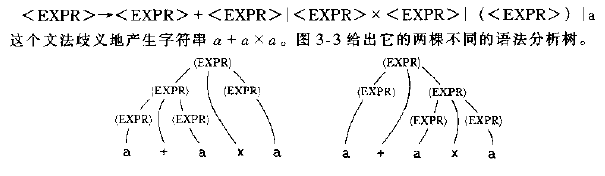
\includegraphics[scale=0.8]{./figure/3.1.4.png}
		\caption{Ambitious grammar}
		\label{F030104}
	\end{figure}

\subsubsection{乔姆斯基范式}

	\colorbox{yellow}{定义3.5} 一个上下文无关文法为\textbf{乔姆斯基范式},如果它的每一个规则具有如下形式:
		$$ A \rightarrow BC $$
		$$ A \rightarrow a $$

	这里,$a$是任意的终结符,$A$、$B$和$C$是任意的变元,但$B$和$C$不能是起始变元。此外,允许规则$S \rightarrow \varepsilon$,其中$S$是起始变元。
	
	\colorbox{green}{定理3.6} 任一上下文无关语言都可以用乔姆斯基范式的上下文无关文法产生。
	
	\textbf{证明思路} \quad 分四阶段将上下文无关语法转化为乔姆斯基范式:
	
	\qquad 1) 增加新的起始变元$S_0$,然后增加规则$S_0 \rightarrow S$。

	\qquad 2) 如果存在$A \rightarrow \varepsilon$,删除这条规则,然后修改其他和$A$有关的规则。
	
	\qquad 3) 处理所有单一规则。对于单一规则$A \rightarrow B$,删除这条,然后增加$A$生成$B$能产生的字符串的规则。举例:对于$A \rightarrow B$和$B \rightarrow u$,删除第一条,增加一条$A \rightarrow u$。
	
	\qquad 4) 把所有留下的规则转换称适当的形式。

\subsection{下推自动机}

\subsubsection{下推自动机的形式定义}

	\colorbox{yellow}{定义3.8} \textbf{下推自动机}是一个$6$元组$(Q,\Sigma,\Gamma,\delta,q_0, F)$,这里$Q$,$\Sigma$,$\Gamma$和$F$都是有穷集合,并且
	
	\qquad 1) $Q$是状态集。
	
	\qquad 2) $\Sigma$是输入字母表。
	
	\qquad 3) $\Gamma$是栈字母表。
	
	\qquad 4) $\delta:Q \times \Sigma_\varepsilon \times \Gamma_\varepsilon \rightarrow \mathcal{P}(Q \times \Gamma_\varepsilon)$
	
	\qquad 5) $q_0 \in Q$是起始状态。
	
	\qquad 6) $F \subseteq Q$是接受状态。

\subsubsection{下推自动机举例}

	\colorbox{pink}{例3.9} 下面是识别语言$\{0^n1^n|n \geq 0\}$的PDA,示意图 \ref{F030202}。
	
	\begin{figure}[htb]
		\centering
		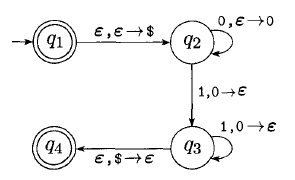
\includegraphics[scale=0.8]{./figure/3.2.2.png}
		\caption{PDA recognizes $\{0^n1^n|n \geq 0\}$}
		\label{F030202}
	\end{figure}

\subsubsection{与上下文无关语法的等价性}

	\colorbox{green}{定理3.12} 一个语言是上下文无关的,当且仅当存在一台下推自动机识别它。
	
	\textbf{证明思路} \quad 使用引理3.13和引理3.15。
	
	\colorbox{cyan}{引理3.13} 如果一个语言是上下文无关的,则存在一台下推自动机识别它。
	
	\textbf{证明思路} \quad 非确定性的枚举,然后压到栈中,和输入进行比较,如果不成立就拒绝该计算分支。如果有一个计算分支接受则接受。
	
	\colorbox{cyan}{引理3.15} 如果一个语言被一台下推自动机识别,则它是上下文无关的。
	
	\textbf{证明思路} \quad 粗略的证明:使用分治的思想,$A_{pq}$可以由$A_{pr}$和$A_{rq}$产生,如图所示\ref{F030203}。
	
	\begin{figure}[htb]
		\centering
		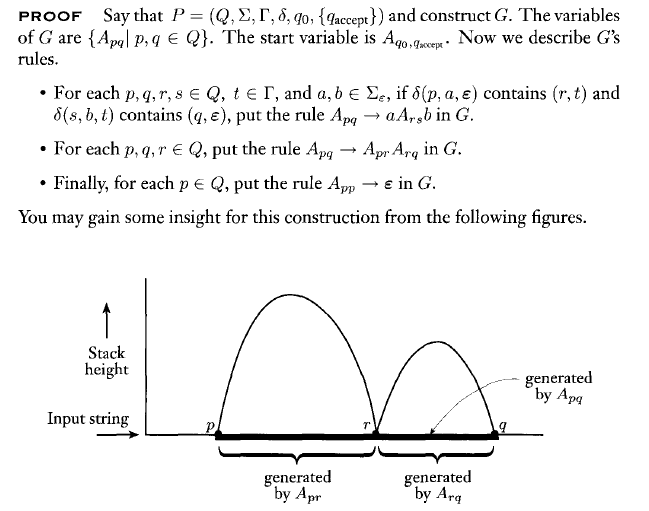
\includegraphics[scale=0.8]{./figure/3.2.3.png}
		\caption{PDA computation corresponding to the rule $A_{pq} \rightarrow A_{pr}A_{rq}$}
		\label{F030203}
	\end{figure}

\subsection{非上下文无关语言}

	\colorbox{green}{定理3.19} (\textbf{关于上下文无关语言的泵引理(Pumping Lemma)})如果$A$是上下文无关语言,则存在数$p$(泵长度Pumping Length),使得$A$中热河一个长度不小于$p$的字符串$s$能够划分成$5$段,$s=uvxyz$,满足下述条件:
	
	\qquad 1) 对于每一个$i$,$uv^ixy^iz \in A$。
	
	\qquad 2) $|vy| > 0$。
	
	\qquad 3) $|vxy| \leq p$。
	
	\textbf{证明思路} \quad 鸽笼原理。取$p=b^{|V|+2}$,其中$b$为一个结点最多的儿子数,$|V|$为$G$中变元的数目(由于叶子节点为终结符,所以这里要加$2$)。示意图 \ref{F030301}。
	
	\begin{figure}[htb]
		\centering
		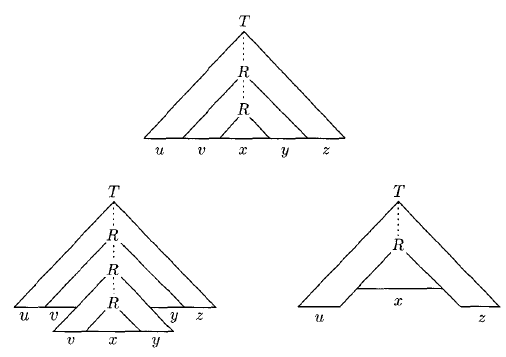
\includegraphics[scale=0.8]{./figure/3.3.1.png}
		\caption{Surgery on parse trees}
		\label{F030301}
	\end{figure}
	
	\colorbox{pink}{例3.20} 用Pumping Lemma证明语言$B=\{a^nb^nc^n|n \geq 0\}$不是上下文无关的。
	
	\textbf{证明}
	
	假设语言$B$是上下文无关的,设Pumping Length为$p$。
	
	令$s=a^pb^pc^p$,则$s$可以被分解为$5$部分,$s=uvxyz$。其中,$|vxy| \leq p$,$|vy|>0$。显然,$vy$中至多包含两种字符。
	
	取$i=0$,即$uv^0xy^0z=uxz$,至少由一种字符的数量减少了,同时至少由一种字符的数量没变。显然,$uxz \notin B$,矛盾!
	
	综上,语言$B$不是上下文无关的。

\section{丘奇—图灵论题}

\subsection{图灵机}

\subsubsection{图灵机的形式定义}

	\colorbox{yellow}{定义4.1} 一个图灵机是一个$7$元组$(Q,\Sigma,\Gamma,\delta,q_0,q_{accept},q_{reject})$,其中:$Q,\Sigma,\Gamma$是有穷集合,并且:
	
	\qquad 1) $Q$是状态集
	
	\qquad 2) $\Sigma$是输入字母表,不包括特殊空白符号。
	
	\qquad 3) $\Gamma$是带字母表,其中:空白符号属于$\Gamma$,$\Sigma \subseteq \Gamma$。
	
	\qquad 4) $\delta:Q \times \Gamma \rightarrow Q \times \Gamma \times \{L,R\}$是转移函数。
	
	\qquad 5) $q_0 \in Q$是起始状态。
	
	\qquad 6) $q_{accept} \in Q$是接受状态。
	
	\qquad 7) $q_{reject} \in Q$是拒绝状态。
	
	图灵机计算时,当前状态、当前带内容和读写头位置,这三项构成的整体叫做图灵机的\textbf{格局}。

	\colorbox{yellow}{定义4.2} 如果有图灵机识别一个语言,则称该语言是\textbf{图灵可识别}的。

	在输入上运行一个TM是,可能出现三种结果:接受、拒绝和循环。\textbf{这里的循环仅仅指机器不停机}。
	
	\colorbox{yellow}{定义4.3} 称一个语言是\textbf{图灵可判定}的,或简单地讲,是\textbf{可判定}的,如果有图灵机判定它。
	
	称对所有输入都停机的图灵机为\textbf{判定器},他们永不循环,总能决定接受还是拒绝。也称识别某个语言的判定器\textbf{判定}该语言。
	
	图灵可判定语言都是图灵可识别语言,但某些图灵可识别语言不是可判定的。

\subsubsection{图灵机的例子}

	\colorbox{pink}{例4.4} 现在描述TM $M_2$,它识别的语言是所有由$0$组成,长度为$2$的放米的字符串,即他判定的语言是$A=\{0^{2^n}|n \geq 0\}$。
	
	$M_2$=“对于输入字符串$w$:
	
	\qquad 1) 从左往右扫描整个带子,隔一个消去一个$0$。
	
	\qquad 2) 如果在第一步之后,带子上只剩下唯一的一个$0$,则接受。
	
	\qquad 3) 如果在第一步之后,带子上包含不只一个$0$,并且$0$的个数是奇数,则拒绝。
	
	\qquad 4) 让读写头返回带子的最左端。
	
	\qquad 5) 转到第一步。”

	下面给出$M_2=(Q, \Sigma, \Gamma, \delta, q_1, q_{accept}, q_{reject})$的形式描述:
	
	\qquad $\bullet$ $Q=\{q_1,q_2,q_3,q_4,q_5,q_{accept},q_{reject}\}$
	
	\qquad $\bullet$ $\Sigma=\{0\}$
	
	\qquad $\bullet$ $\Gamma=\{0,x,BLANK\}$
	
	\qquad $\bullet$ 将$\delta$描述成状态图 \ref{F040102}
	
	\qquad $\bullet$ 开始、接受和拒绝状态分别是$q_1$、$q_{accept}$和$q_{reject}$。
	
	\begin{figure}[htb]
		\centering
		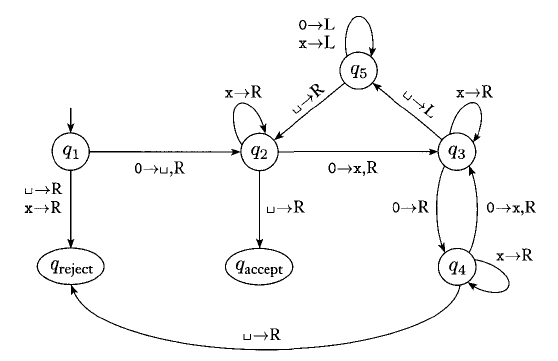
\includegraphics[scale=0.8]{./figure/4.1.2.png}
		\caption{State diagram for Turing machine $M_2$}
		\label{F040102}
	\end{figure}

\subsection{图灵机的变形}

\subsubsection{多带图灵机}

	\textbf{多带图灵机},在普通图灵机的基础上,有多个带子,每个带子都有子集的读写头,用于读和写。开始时,输入出现在第一个带子上,其余的带子都是空白的。转移函数该为允许同时进行读、写和移动读写头,其形式为:
	$$\delta:Q \times \Gamma^k \rightarrow Q \times \Gamma^k \times \{L,R\}^k$$

	\colorbox{green}{定理4.8} 每个多带图灵机都有一个与之等价的单带图灵机。
	
	\textbf{证明思路} \quad 把多条纸带的内容写道一条纸带上,用特殊符号分隔。

	\colorbox{gray}{推论4.9} 一个语言是图灵可识别的,当且仅当有多带图灵机识别它。
	
	\textbf{证明思路} \quad 多带图灵机可以转化为单带图灵机。

\subsubsection{非确定型图灵机}

	\textbf{非确定型图灵机},在计算的任何时刻,机器可以在多种可能性中选择一种继续进行,它的转移函数具有如下形式:
	$$\delta: Q \times \Gamma \rightarrow \mathcal{P}_3(Q \times \Gamma \times \{L,R,S\})$$

	\colorbox{green}{定理4.10} 每个非确定型图灵机都有一个与之等价的确定型图灵机。
	
	\textbf{证明思路} \quad 使用宽度优先搜索的方法(BFS)模拟非确定型的计算分支,一共使用三条纸带。
	
	\qquad 1)第一条纸带用于储存输入,只读不写。
	
	\qquad 2)第二条纸带用于进行与原来NTM类似的计算。
	
	\qquad 3)第三条纸带用与存储可能转移到的下一组格局。

	\colorbox{gray}{推论4.11} 一个语言是图灵可识别的,当且仅当有非确定型图灵机识别它。
	
	\textbf{证明思路} \quad 非确定型图灵机能转化为多带图灵机,多带图灵机可以转化为单带图灵机。
	
	\colorbox{gray}{推论4.12} 一个语言是可判定的,当且仅当有非确定型图灵机判定它。

\subsubsection{枚举器}

	\colorbox{green}{定理4.13} 一个语言是图灵可识别的,当且仅当有枚举器枚举它。
	
	\textbf{证明思路}
	
	如果有枚举器$E$枚举语言$A$,则有TM$M$识别$A$。TM$M$如下运行:
	
	$M$=“对与输入$w$:
	
	\qquad 1) 运行$E$,每当$E$输出一个串时,将之与$w$比较。
	
	\qquad 2) 如果$w$曾经在$E$的输出中出现过,则接受。”

	如果TM$M$识别语言$A$,为$A$构造枚举器$E$如下:
	
	$E$=“忽略输入。
	
	\qquad 1) 对$i=1,2.3,\dots$重复下列步骤。
	
	\qquad 2) 对$s_1,s_2,\dots,s_i$中的每一个,让$M$以其作为输入运行$i$步。
	
	\qquad 3) 如果有计算接受,则打印出相应的$s_j$。

\subsubsection{与其他模型的等价性}

	略

\subsection{算法的定义}

\subsubsection{希尔伯特问题}

	\textbf{希尔伯特问题}
	$$D=\{p|p~is~a~polynomial~with~an~integral~root\}$$

	对于一元多项式,其根在$\pm k\frac{c_{max}}{c_1}$。其中,$k$是此多项式中项的个数,$c_{max}$是绝对值最大的系数,$c_1$是最高次项的系数。因此,一元多项式是否有整数根的问题是可判定的。
	
	但是,多元多项式是否有整数根的问题是不可判定的。

\subsubsection{描述图灵机的术语}

	略。

\section{可判定性}

\subsection{可判定语言}

\subsubsection{与正则语言相关的可判定性}

	\colorbox{green}{定理5.1} $A_{DFA}=\{<B,w>|B~is~DFA,~w~is~string,~B~accepts~w\}$是一个可判定语言。
	
	\textbf{证明思路} \quad 在输入$w$上模拟$B$即可。
	
	\colorbox{green}{定理5.2} $A_{NFA}=\{<B,w>|B~is~NFA,~w~is~string,~B~accepts~w\}$是一个可判定语言。
	
	\textbf{证明思路} \quad 先将NFA转化为DFA,然后在输入上模拟即可。
	
	\colorbox{green}{定理5.3} $A_{REX}=\{<B,w>|B~is~regular~expression~that~generates~string~w\}$是一个可判定语言。
	
	\textbf{证明思路} \quad 先将正则表达式转化为DFA,然后在输入上模拟即可。
	
	\colorbox{green}{定理5.4} $E_{DFA}=\{<A>|A~is~a~DFA~and~L(A)=\emptyset\}$是一个可判定语言。
	
	\textbf{证明思路} \quad 从DFA的起始状态开始遍历,如果不能到达接受状态就接受,否则就拒绝。

	\colorbox{green}{定理5.5} $EQ_{DFA}=\{<A,B>|A~and~B~are~DFAs~and~L(A)=L(B)\}$是一个可判定语言。
	
	\textbf{证明思路} \quad 构造DFA$C$,满足$L(C)=(L(A) \cap \overline{L(B)}) \cup (\overline{L(A)} \cap L(B))$。判断$L(C)$是否为空,为空则接受,否则拒绝。构造$L(C)$的时候转化成正则表达式,正则语言类在补、并和交下是封闭的。

\subsubsection{与上下文无关语言相关的可判定性问题}

	\colorbox{green}{定理5.6} $A_{CFG}=\{<G,w>|G~is~a~CFG~that~generates~string~w\}$是一个可判定语言。
	
	\textbf{证明思路} \quad 转成乔姆斯基文法,列出$2n-1$步的所有派生($n$为$w$的长度),判断$w$是否在其中。
	
	\colorbox{green}{定理5.7} $E_{CFG}=\{<G>|G~is~a~CFG~and~L(G)=\emptyset\}$是一个可判定语言。
	
	\textbf{证明思路} \quad 把终结符都打上标记,然后对于规则$A \rightarrow U_1 \dots U_k$,如果$U_1,\dots,U_k$都有标记,就把$A$也打上标记。如果起始状态没被标记则接受,否则拒绝。
	
	\colorbox{green}{定理5.8} 每个上下文无关语言是可判定的。
	
	\textbf{证明思路} \quad 使用定理5.6提到的图灵机。

\subsection{停机问题}

	\colorbox{green}{定理5.9} $A_{TM}=\{<M,w>|M~is~a~TM~that~accepts~w\}$是不可判定的。
	
	$A_{TM}$有时被成为停机问题。

\subsubsection{对角化方法}

	\colorbox{yellow}{定义5.10} 设$A$和$B$两个集合,$f$是从$A$到$B$的函数。如果$f$从步将两个不同元素映射到同一地方,即:只要$a \neq b$就有$f(a) \neq f(b)$,则称$f$是\textbf{一对一}的。对于$B$中的每个元素$b$,都存在$a \in A$,使得$f(a)=b$,则称$f$是\textbf{到上的}。如果一个函数即使一对一又是到上的,那么称为\textbf{对应}。
	
	\colorbox{pink}{例5.11} 自然数集合$\mathcal{N}=\{1,2,3,\dots\}$和偶自然数集合$\varepsilon=\{2,4,6,\dots\}$具有相同的规模。
	
	\colorbox{yellow}{定义5.12} 成一个集合是可数的,如果它是有限的,或者它与$\mathcal{N}$有相同的规模。

	\colorbox{pink}{例5.13} 正有理数集合$\mathcal{Q}$与自然数集合$\mathcal{N}$具有相同的规模,示意图 \ref{F050201}。
	
	\begin{figure}[htb]
		\centering
		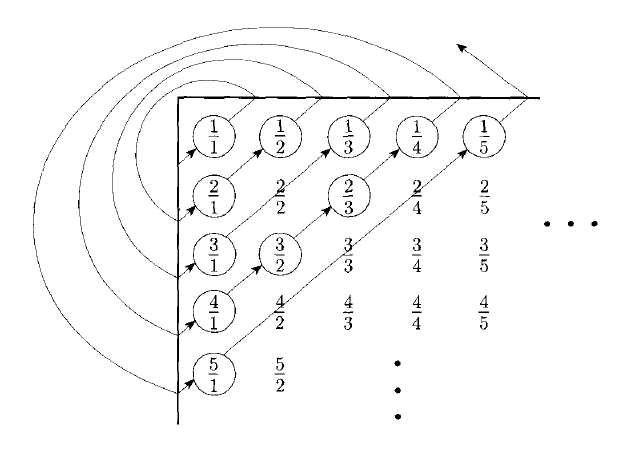
\includegraphics[scale=0.8]{./figure/5.2.1.png}
		\caption{A correspondence of $\mathcal{N}$ and $\mathcal{Q}$}
		\label{F050201}
	\end{figure}
	
	\colorbox{green}{定理5.14} $\mathcal{R}$是不可数的。
	
	\textbf{证明思路} \quad 假设每个自然数都对应了一个实数,那么取$x \in \mathcal{R}$,其中$x$的整数位为0,第$i$位小数与自然数$i$的第$i$位小数不同。因此,该实数没有被任意一个自然数映射。

	\colorbox{gray}{推论5.15} 存在语言不是图灵可识别的。
	
	\textbf{证明思路} \quad 证明分为两部分:
	
	\qquad 1) 所有图灵机构成的集合是可数的。
	
	\qquad 2) 所有语言构成的集合是不可数的。

\subsubsection{停机问题是不可判定的}
	
	\textbf{证明}
	
	假设$A_{TM}$是可判定的。设$H$是$A_{TM}$的判定器。令$M$是一个TM,$w$是一个串。
		$$H(<M,w>)=
		\begin{cases}
			accept& \text{M accepts w}\\
			reject& \text{M rejects w}
		\end{cases}$$
		
	构造一个新的图灵机$D$,输入为一个图灵机$M$。在输入$<M,<M>>$上运行$H$,并且得出与$H$相反的结论。
	
	当以$D$的描述$<D>$作为输入来运行$D$自身时,有
		$$D(<D>)=
		\begin{cases}
			accept& \text{D rejects <D>}\\
			reject& \text{D accepts <D>}
		\end{cases}$$
	
	矛盾!
	
	综上,图灵机$H$是不存在的。
	
\subsubsection{一个图灵不可识别语言}

	\colorbox{green}{定理5.16} 一个语言是可判定的,当且仅当它既是图灵可识别的,也是补图灵可识别的。
	
	\textbf{证明思路} 证明分两个部分:
	
	\qquad 1) 如果$A$是可判定的,显然$A$和$\overline{A}$都是图灵可识别的。因为任何可判定语言都是图灵可识别语言,任何可判定语言的补都是可判定语言。
	
	\qquad 2) 构造两个图灵机:$M_1$识别$A$,$M_2$识别$\overline{A}$。构造图灵机$M$:在$M_1$和$M_2$上同时运行$A$(可以采用多带图灵机)。如果$M_1$接受就接受,$M_2$接受就拒绝。
	
	\colorbox{gray}{推论5.17} $\overline{A_{TM}}$不是图灵可识别的。
	
	\textbf{证明思路} \quad 如果$\overline{A_{TM}}$是图灵可识别的,那么可以推出$A_{TM}$是可判定的,矛盾!

\section{可归约性}

\subsection{语言理论中的不可判定问题}

	\colorbox{green}{定理6.1} $HALT_{TM}=\{<M,w>|M~is~a~TM~and~M~halts~on~input~s\}$是不可判定的。
	
	\textbf{证明思路} \quad 用反证法,$A_{TM}$可以归约到$HALT_{TM}$。
	
	\colorbox{green}{定理6.2} $E_{TM}=\{<M>|M~is~a~TM~and~L(M)=\emptyset\}$是不可判定的。
	
	\textbf{证明思路} \quad 用反证法,把$A_{TM}$归约到$E_{TM}$。对于一个TM,先判断输入是否为$w$,如果不是直接拒绝,否则执行图灵机。如果$E_{TM}$可判定,那么$A_{TM}$也是可判定的。
	
	\colorbox{green}{定理6.3} $REGULAR_{TM}=\{<M>|M~is~a~TM~and~L(M)~is~a~regular~language\}$是不可判定的。
	
	\textbf{证明思路} \quad 用反证法,如果$REGULAR_{TM}$是可判定的,那么$A_{TM}$也是可判定的。
	
	设判定$REGULAR_{TM}$的图灵机为$R$,判定$A_{TM}$的图灵机为$S$。对于输入$<M,w>$,构造图灵机$M_2$,如果输入为$0^n1^n$的形式,则接受。否则,在输入$w$上运行$M$,$M$接受$M_2$就接受,否则拒绝。在输入$<M_2>$上运行$R$,如果$R$接受则$S$接受,否则拒绝。

	\colorbox{green}{补充定理} \textbf{Race Theorem} Let P be any problem about TM that satisfies the following two properties. As usual, P is expressed as a language.

	\qquad 1) For any TMs $M_1$ and $M_2$, where $L(M_1)=L(M_2)$, we have $<M_1>\in P \Leftrightarrow <M_2>\in P$
	
	\qquad 2) There exist TMs $M_1$ and $M_2$, where $<M_1>\in P$, $<M_2>\notin P$.
	
	Then \color{red} P is undecidable \color{black}.

	\colorbox{green}{定理6.4} $EQ_{TM}=\{<M_1,M_2>|M_1~and~M_2~are~TMs~and~L(M_1)=L(M_2)\}$是不可判定的。
	
	\textbf{证明思路} \quad 用反证法,在输入$<M,M_1>$上运行$EQ_{TM}$,其中$M_1$拒绝所有输入,即可判定$E_{TM}$问题,矛盾。
	
	\colorbox{yellow}{定义6.5} 设$M$是一个图灵机,$w$是一个串。$M$在$w$上的一个\textbf{接受计算历史}是一个格局序列$C_1,C_2,\dots,C_l$,其中:$C_1$是$M$在$w$上的其实格局,$C_l$是$M$的一个接受格局,且每个$C_i$都是$C_{i-1}$的合法结果,即符合$M$的规则。同理可以定义\textbf{拒绝计算历史}。

	\colorbox{yellow}{定义6.6} \textbf{线性界限自动机(LBA)} 是一种受到限制的图灵机,它不允许其读写头离开包含输入的带区域。
	
	\colorbox{cyan}{引理6.7} 设$M$是有$q$个状态和$g$个带符号的$LBA$。对于长度为$n$的带子,$M$汽油$qng^n$个不同的格局。
	
	\textbf{证明思路} \quad 每个状态、读写头位置、纸带内容。
	
	\colorbox{green}{定理6.8} $A_{LBA}=\{<M,w>|M~is~a~LBA~that~accepts~w\}$是可判定的。

	\textbf{证明思路} \quad 因为LBA的格局数有限,当模拟超过一定步数后,会出现循环,直接拒绝。这样保证了一定能停机。
	
	\colorbox{green}{定理6.9} $E_{LBA}=\{<M>|M~is~a~LBA~and~L(M)=\emptyset\}$是不可判定的。
	
	\textbf{证明思路} \quad 构造$A_{TM}$的判定机$R$。对于输入$<M,w>$,构造一个接受$<M,w>$的接受计算历史的LBA$B$。如果$B$接受的语言为空,$R$则拒绝,否则接受。

	\colorbox{green}{定理6.10} $ALL_{CFG}=\{<G>|G~is~a~CFG~and~L(G)=\Sigma^*\}$是不可判定的。
	
	\textbf{证明思路} \quad 对于$<M,w>$,构造CFG派生所有计算历史(\textbf{除了接受计算历史})。如果CFG能接受所有串,那么$M$就不能接受$w$,否则$M$就能接受$w$。

	可以用定理6.10来证明\textbf{$EQ_{CFG}$是不可判定的}。

\subsection{一个简单的不可判定问题}

	一个关于串操作的不可判定问题,称为\textbf{波斯特对应问题},或\textbf{PCP}。
	
	一族骨牌:
	$$\{[\frac{b}{ca}],[\frac{a}{ab}],[\frac{ca}{a}],[\frac{abc}{c}]\}$$
	
	上述骨牌的一个匹配:
	$$[\frac{a}{ab}],[\frac{b}{ca}],[\frac{ca}{a}],[\frac{a}{ab}],[\frac{abc}{c}]$$
	
	骨牌的上部和下部组成的字符串都是$abcaaabc$。

	\colorbox{green}{定理6.11} $PCP=\{<P>|P~is~an~instance~of~the~PCP~with~a~match\}$是不可判定的。
	
	\textbf{证明思路} \quad 用反证法,利用$PCP$问题,构造判定$A_{TM}$问题的图灵机。
	
	先将$PCP$问题转化为$MPCP$问题(第一个骨牌是固定的),利用接受历史计算来构造骨牌的上部(上一个历史计算)和下部(下一个历史理算)。如果有一个匹配,就是有一个接受历史计算,示意图 \ref{F060201}。

	\begin{figure}[htb]
		\centering
		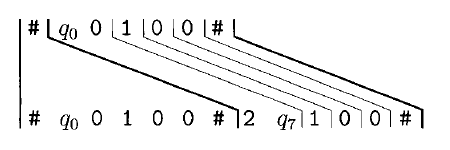
\includegraphics[scale=0.8]{./figure/6.2-1.png}
		\caption{Example of $MPCP$}
		\label{F060201}
	\end{figure}

	通过添加特殊符号,将$MPCP$问题转化为$PCP$问题,示意图 \ref{F060202}。

	\begin{figure}[htb]
		\centering
		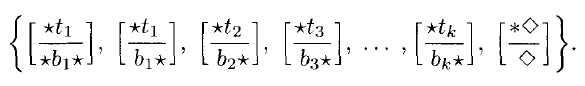
\includegraphics[scale=0.8]{./figure/6.2-2.png}
		\caption{$MPCP$ to $PCP$}
		\label{F060202}
	\end{figure}
	

\subsection{映射可归约性}

	用映射可归约性将问题$A$归约为问题$B$。

\subsubsection{可计算函数}

	\colorbox{yellow}{定义6.12} 函数$f:\Sigma^* \rightarrow \Sigma^*$是一个可计算函数,如果有某个图灵机$M$,使得在每个输入$w$上,$M$停机,且此时只有$f(w)$出现在带上。

\subsubsection{映射可归约的形式定义}

	\colorbox{yellow}{定义6.15} 语言$A$是\textbf{映射可归约}到语言$B$的,如果存在可计算函数$f:\Sigma^* \rightarrow \Sigma^*$使得对每个$w$,
	$$w \in A \Leftrightarrow f(w) \in B$$
	
	记作$A \leq_m B$。称函数$f$为$A$到$B$的归约。

	\colorbox{green}{定理6.16} 如果$A \leq_m B$且$B$是可判定的,则$A$也是可判定的。
	
	\colorbox{gray}{推论6.17} 如果$A \leq_m B$且$A$不是可判定的,则$B$也不是可判定的。

	\colorbox{green}{定理6.22} 如果$A \leq_m B$且$B$是图灵可识别的的,则$A$也是图灵可识别的的。
	
	\colorbox{gray}{推论6.23} 如果$A \leq_m B$且$A$不是图灵可识别的,则$B$也不是图灵可识别的。
	
	\colorbox{green}{定理6.24} $EQ_{TM}$既不是图灵可识别的,也不是不图灵可识别的。
	
	\textbf{证明思路} \quad 分为两步
	
	\qquad 1) 证明$EQ_{TM}$不是图灵可识别的,只要证明$A_{TM}$可归约到$\overline{EQ_{TM}}$即可。
	
	\qquad 2) 证明$\overline{EQ_{TM}}$不是图灵可识别的,只要证明$A_{TM}$可归约到$\overline{\overline{EQ_{TM}}}$即可。

\section{可计算理论的高级专题}

\subsection{递归定理}

\subsubsection{自引用}

	\colorbox{cyan}{引理7.1} 存在可计算函数$q:\Sigma^* \rightarrow \Sigma^*$,对任意串$w$,q(w)是图灵机$P_w$的描述,$P_w$打印出$w$,然后停机。

	输出图灵机自己的编码,可以将这个编码分为两部分:$<SELF>=<AB>$。首先,令$<A>=q(<B>)$,然后$A$输出$<B>$,接着$B$根据$<B>$输出$q(<B>)$,最后拼接得到$<AB>=<SELF>$。

	\colorbox{green}{定理7.2} \textbf{递归定理} \quad 设$T$是计算函数$t:\Sigma^* \rightarrow \Sigma^*$的一个图灵机。则存在计算函数$r:\Sigma^* \rightarrow \Sigma^*$的一个图灵机$R$,使得对每个$w$,有:
	$$r(w)=t(<R>,w)$$

\subsubsection{应用递归定理的术语}

	略

\subsubsection{应用}

	\colorbox{green}{定理7.3} $A_{TM}$是不可判定的。
	
	\textbf{证明思路} \quad 反证法。假设图灵机$H$判定$A_{TM}$,构造图灵机$B$:对于输入$w$,通过递归定理构造$<B>$,在输入$<B,w>$上运行$H$。如果$H$接受,则$B$拒绝;如果$H$拒绝,则$B$接受。

	\colorbox{yellow}{定义7.4} 如果$M$是一个图灵机,则$M$的描述$<M>$的\textbf{长度}是描述$M$的串中所含符号的个数。如果没有与$M$等价的图灵机有更短的描述,则称$M$是\textbf{极小的}。令
	$$MIN_{TM}=\{<M>|M~is~a~minimal~TM\}$$

	\colorbox{green}{定理7.5} $MIN_{TM}$是不可判定的。
	
	\textbf{证明思路} \quad 反证法。假设TM$E$枚举$MIN_{TM}$,构造TM$C$:对于任意输入$w$,通过递归定理得到自己的描述$<C>$,然后通过枚举器$E$找到一个更长描述的TM$D$,在$w$上模拟$D$。如果$D$接受,$C$就接受;如果$D$拒绝,$C$就拒绝。
	
	\colorbox{green}{定理7.6} 设$t:\Sigma^* \rightarrow \Sigma^*$是一个可计算函数,则存在一个图灵机$F$,使得$t(<F>)$描述一个与$F$等价的图灵机。
	
	\textbf{证明思路} \quad 构造图灵机$F$:对于任意输入$w$,通过递归定理获得自己的描述$<F>$,然后计算$t(<F>)$得到一个TM$G$的描述,在输入$w$上模拟$G$。如果$G$接受,$F$就接受;如果$G$拒绝,$F$就拒绝。

\subsection{逻辑理论的可判定性}

	对于模型$\mathcal{M}$,令$\mathcal{M}$的理论是这个模型语言中所有真聚集的集合,记作$Th(\mathcal{M})$。

\subsubsection{一个可判定的理论}

	\colorbox{green}{定理7.10} $Th(\mathcal{N},+)$是可判定的。

\subsubsection{一个不可判定的理论}

	\colorbox{green}{定理7.11} $Th(\mathcal{N},+, \times)$是不可判定的。
	
	\colorbox{cyan}{引理7.12} 设$M$是一个图灵机,$w$是一个串。从$M$和$w$能构造$Th(\mathcal{N},+, \times)$的语言中的公式$\phi_{M,w}$,使得它只包含单个自由变元$x$,且句子$\exists x \phi_{M,w}$为真当且仅当$M$接受$w$。

	\colorbox{green}{定理7.13} $Th(\mathcal{N},+, \times)$中可证命题的集合是图灵可识别的。
	
	\colorbox{green}{定理7.14} $Th(\mathcal{N},+, \times)$中有真命题是不可证的。

\subsection{图灵可归约性}

	\colorbox{yellow}{定义7.16} 语言$B$的一个\textbf{谕示}是一个能够报告某个串是否为$B$的成员的外部装置。一个\textbf{谕示图灵机}是一种修改过的图灵机,它有询问一个谕示的额外能力。记$M^B$为对语言$B$有谕示的谕示图灵机。
	
	\colorbox{yellow}{定义7.19} 语言$A$\textbf{图灵可归纳}到$B$,如果$A$相对于$B$是可判定的,基座$A \leq_T B$。
		
	\colorbox{green}{定理7.19} 如果$A \leq_T B$且$B$是可判定的,则$A$也是可判定的。

\subsection{信息的定义}

\subsubsection{极小长度的描述}

	\colorbox{yellow}{定义7.20} 设$x$是二进制数的串。$x$的\textbf{极小描述}是最短的串$<M,w>$,其中:TM$M$在输入$w$上停机时,$x$在带上。且如果有多个这样的串存在,则在其中选择字典序下的第一个串。记$x$的极小描述为$d(x)$。$x$的\textbf{描述复杂性}$K(x)$是
	$$K(x)=|d(x)|$$

	\colorbox{green}{定理7.21} $\exists c \forall x [K(x) \leq |x| + c]$
	
	\colorbox{green}{定理7.22} $\exists c \forall x [K(xx) \leq K(x) + c]$
	
	\colorbox{green}{定理7.23} $\exists c \forall x, y [K(xy) \leq 2K(x) + K(y) + c]$

\subsubsection{定义的优化}

	\colorbox{green}{定理7.24} 对任何描述语言$p$,存在一个只与$p$有关的常量$c$,使得:
	$$\forall x[K(x) \leq K_p(x)+c]$$

\subsubsection{不可压缩的串和随机性}

	\colorbox{yellow}{定义7.25} 设$x$是一个串。如果
	$$K(x) \leq |x|-c$$
	
	则称$x$是\textbf{$c$—可压缩的}。如果$x$不是\textbf{$c$—可压缩的},则称$x$是\textbf{不可压缩$c$的}。如果$x$是不可压缩$1$的,则称$x$是\textbf{不可压缩的}。
	
	\colorbox{green}{定理7.26} 对于每个长度,都存在不可压缩的串。
	
	\colorbox{gray}{推论7.27} 至少有$2^n-2^{n-c+1}+1$个长度为$n$的串是不可压缩$c$的。

	\colorbox{green}{定理7.28} 设$f$是一个对几乎所有串成立的性质,则对任意$b>0$,性质$f$只在有限多个不可压缩$b$的串上的值是FALSE。
	
	\colorbox{green}{定理7.29} 存在常量$b$,使得对每个串$x$,$x$的极小描述$d(x)$都不可压缩$b$。

\section{时间复杂性}

\subsection{度量复杂性}

	\colorbox{yellow}{定义8.1} 时间复杂度是一个函数:$f: \mathcal{N} \rightarrow \mathcal{N}$。
	
\subsubsection{大$O$和小$o$记法}

	\colorbox{yellow}{定义8.2} 设$f$和$g$是两个函数$f,g:\mathcal{N} \rightarrow \mathcal{R}^+$。称$f(n)=O(g(n))$,若存在正整数$c$和$n_0$,使得对所有$n\geq n_0$,有
	$$f(n)\leq cg(n)$$
	
	当$f(n)=O(g(n))$时,称$g(n)$是$f(n)$的\textbf{上界},更准确说是\textbf{渐进上界}。
	
	\colorbox{pink}{例8.3} 设$f_1(n)=5n^3+2n^2+22n+6$,则$f_1(n)=O(n^3)$
	
	\colorbox{pink}{例8.4} 写$f(n)=O(\log{n})$时,不必再指明基数。
	
	\colorbox{yellow}{定义8.5} 设$f$和$g$是两个函数$f,g:\mathcal{N} \rightarrow \mathcal{R}^+$。称$f(n)=o(g(n))$,若存在正整数$n_0$,对于任何实数$c>0$,使得对所有$n\geq n_0$,有
	$$f(n) < cg(n)$$
	
	或
	$$\lim_{n \rightarrow \infty} \frac{f(n)}{g(n)}=0$$
	
\subsubsection{分析算法}

	对于语言$A=\{0^k1^k|k \geq 0\}$,算法如图所示 \ref{F080102}。该算法的时间复杂度为$O(n^2)$
	
	\begin{figure}[htb]
		\centering
		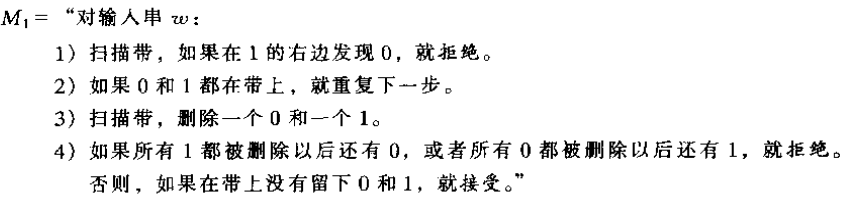
\includegraphics[scale=0.8]{./figure/8.1.2.png}
		\caption{Algorithm~for~language~$A=\{0^k1^k|k \geq 0\}$}
		\label{F080102}
   \end{figure} 
   
   \colorbox{yellow}{定义8.7} 令$t:\mathcal{N} \rightarrow \mathcal{N}$是一个函数。定义时间复杂性类$TIME(t(n))$为
   $$TIME(t(n))=\{L|L~is~a~language~that~can~be~decided~in~O(t(n))\}$$

	对于语言$A$存在一个$O(n\log{n})$的算法:每次间隔一个删一个,直至删完。
	
	当图灵机有两条纸带时,语言$A$能在$O(n)$的时间内被判定。
   
\subsubsection{模型间的复杂度关系}

	\colorbox{green}{定理8.8} 设$t(n)$是一个函数,$t(n) \geq n$。则每一个$t(n)$时间的多带图灵机都和某一个$O(t(n)^2)$时间的单带图灵机等价。
	
	\textbf{证明思路} \quad 模拟多带图灵机的每一步最多需要单带机的$O(t(n))$步,因此总共需要时间为$O(t^2(n))$步。

	\colorbox{yellow}{定义8.9} $N$的运行时间是函数$f:\mathcal{N} \rightarrow \mathcal{N}$,$f(n)$是在任何长度为$n$的输入上,$N$的所有计算分支的最大步数。
	
	\colorbox{green}{定理8.10} 设$t(n)$是一个函数,$t(n) \geq n$。则每一个$t(n)$时间的非确定型单带图灵机都和某一个$2^{O(t(n)^2)}$时间的确定型单带图灵机等价。
	
	\textbf{证明思路} \quad 对递归模拟计算树。计算树的最大深度为$O(t(n))$,最后一层有$b$个儿子,则$O(t(n)b^{t(n)})=2^{O(t(n))}$

\subsection{$P$类}

\subsubsection{多项式时间}

	\colorbox{yellow}{定义8.11} $P$是确定型单带图灵机在多项式时间内可判定的语言类。换句话说,
	$$P=\cup_k(n^k)$$

\subsubsection{$P$中的问题举例}

	$PATH=\{<G,s,t>|G~is~a~directed~graph~that~has~a~directed~path~from~s~to~t\}$

	\colorbox{green}{定理8.12} $PATH \in P$。

	$RELPRIME=\{<x,y>| x~and~y~are~relatively~prime\}$
	
	\colorbox{green}{定理8.13} $RELPRIME \in P$。
	
	\colorbox{green}{定理8.14} 每一个上下文无关语言都是$P$的成员。
	
	\textbf{证明思路} \quad 对于一个$CFL$,存在对应的乔姆斯基范式$G$。对于长度为$n$的串,需要$2n-1$来生成。使用动态规划算法进行判定,运行时间为$O(n^3)$。

\subsection{$NP$类}

	\colorbox{yellow}{定义8.15} 语言$A$的验证机是一个算法$V$,这里
	$$A=\{w|V~accepts~<w,c>~for~some~string~c\}$$
	
	\colorbox{yellow}{定义8.16} $NP$是具有多项式时间验证机的语言类。

	\colorbox{green}{定理8.17} 一个语言在$NP$中,当且仅当它能被某个非确定型多项式图灵机判定。
	
	\textbf{证明思路} \quad 非确定性地枚举证书进行验证。

	\colorbox{yellow}{定义8.18}
	$$NTIME(t(n))=\{L|L~is~a~language~decided~by~a~O(t(n))~time~nondeterministic~Turing~machine\}$$

	\colorbox{gray}{推论8.19} $NP=\cup_k NTIME(n^k)$

\subsubsection{$NP$中的问题举例}

	$CLIQUE=\{<G,k>|G~is~an~undirected~graph~with~a~k-clique\}$

	\colorbox{green}{定理8.20} $CLIQUE$属于$NP$。
	
	\textbf{证明思路} 
	
		\qquad \textbf{思路一:} 团即是证书。
		
		\qquad \textbf{思路二:} 非确定性地选择一个点集,验证这个点集是否满足条件。

	\begin{multline}
		SUBSET-SUM=\{<S,t>|S=\{x_1,\dots,x_k\}~and~for~some \\
							\{y_1,\dots,y_l\}\subseteq S,~we~have~\Sigma{y_i}=t\}
	\end{multline}
	
	\colorbox{green}{定理8.21} $SUBSET-SUM$属于$NP$。

	\textbf{证明思路} 子集即是证书。

\subsubsection{$P$与$NP$问题}

	求解$NP$语言的已知的最好方式确定性地使用指数时间。换言之,可以证明。
	$$NP \subseteq EXPTIME=\cup_k TIME(2^K)$$

\subsection{$NP$完全性}

	$SAT=\{<\phi>|\phi~is~a~satisfiable~Boolean~formula\}$

	\colorbox{green}{定理8.22} 库克—列文定理
	$$SAT \in P~if~and~only~if~P=NP$$

\subsubsection{多项式时间可归约性}

	\colorbox{yellow}{定义8.23} 若存在多项式时间图灵机$M$,使得在任何输入$w$上,$M$停机是$f(w)$恰好在带上,则称函数$f:\Sigma^* \rightarrow \Sigma^*$为\textbf{多项式时间可计算函数}。
	
	\colorbox{yellow}{定义8.24} 语言$A$成为多项式时间映射可归约到语言$B$,或简称为多项式时间可归约到$B$,记为$A\leq_P B$,若存在多项式时间可计算函数:$f:\Sigma^* \rightarrow \Sigma^*$,对于每一个$w$,有
	$$w \in A \Leftrightarrow f(w) \in B$$
函数$f$称为$A$到$B$的\textbf{多项式归约}。

	\colorbox{green}{定理8.25} 若$A \leq_P B$且$B \in P$,则$A \in P$。
	
	\textbf{证明思路} \quad $A$多项式时间归约到$B$,然后$B$在多项式时间内求解。
	
	\colorbox{green}{定理8.26} $3SAT$多项式时间可规约到$CLIQUE$。
	
	\textbf{证明思路} \quad 可以同时成真的结点连边,需要找一个大小为$k$的团($k$为合取式的数量),示意图 \ref{F080401}

	\begin{figure}[htb]
		\centering
		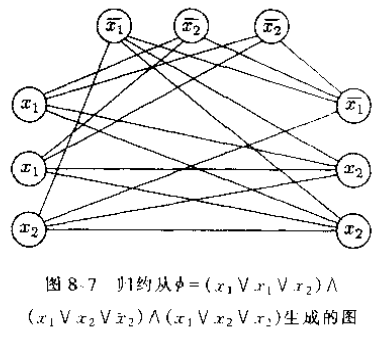
\includegraphics[scale=0.8]{./figure/8.4.1.png}
		\caption{$3SAT$~to~$CLIQUE$}
		\label{F080401}
   \end{figure} 

\subsubsection{$NP$完全性的定义}

	\colorbox{yellow}{定义8.27} 语言$B$是\textbf{$NP$完全的},若它满足两个条件:
	
	\qquad \textbf{1)} $B$属于$NP$。

	\qquad \textbf{2)} $NP$中的每一个语言$A$多项式时间可归约到$B$。
	
	\colorbox{green}{定理8.28} 若$B$是$NP$完全的,且$B \in P$,则$P=NP$。
	
	\colorbox{green}{定理8.29} 若$B$是$NP$完全的,且$B \leq_P C$,$C$属于$NP$,则$C$是$NP$完全的。

\subsubsection{库克—列文定理}

	\colorbox{green}{定理8.30} $SAT$是$NP$完全的。
	
	\textbf{证明思路} \quad 首先,证明$SAT$是$NP$的(容易)。然后证明所有$NP$的问题都能规约到$SAT$(极其困难,略)。
	
	\colorbox{gray}{推论8.32} $3SAT$是$NP$完全的。
	
	要证明一个问题是$NP$完全的,只需证$3SAT$能归约到这个问题,且这个问题是$NP$的即可。

\subsection{几个$NP$完全问题}

	\colorbox{gray}{推论8.33} $CLIQUE$是$NP$完全的。

\subsubsection{顶点覆盖问题}
	
	\begin{multline}
		VECTOR-COVER=\{<G,k>|G~is~an~undirected~graph~that \\
							has~a~k-node~vertex~cover\}
	\end{multline}
	
	\colorbox{green}{定理8.34} $VECTOR-COVER$是$NP$完全的。
	
	\textbf{证明思路} \quad 从$3SAT$归约到$VECTOR-COVER$,示意图 \ref{F080501}。

	\begin{figure}[htb]
		\centering
		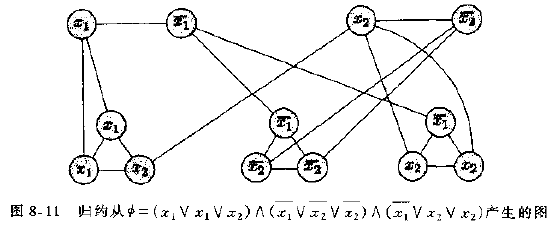
\includegraphics[scale=0.8]{./figure/8.5.1.png}
		\caption{$3SAT$~to~$VECTOR-COVER$}
		\label{F080501}
   \end{figure} 

\subsubsection{哈密顿路径问题}

	\colorbox{green}{定理8.35} $HAMPATH$是$NP$完全的。
	
	\textbf{证明思路} \quad 从$3SAT$归约到$HAMPATH$,示意图 \ref{F080502}。
	
	\begin{figure}[htb]
		\centering
		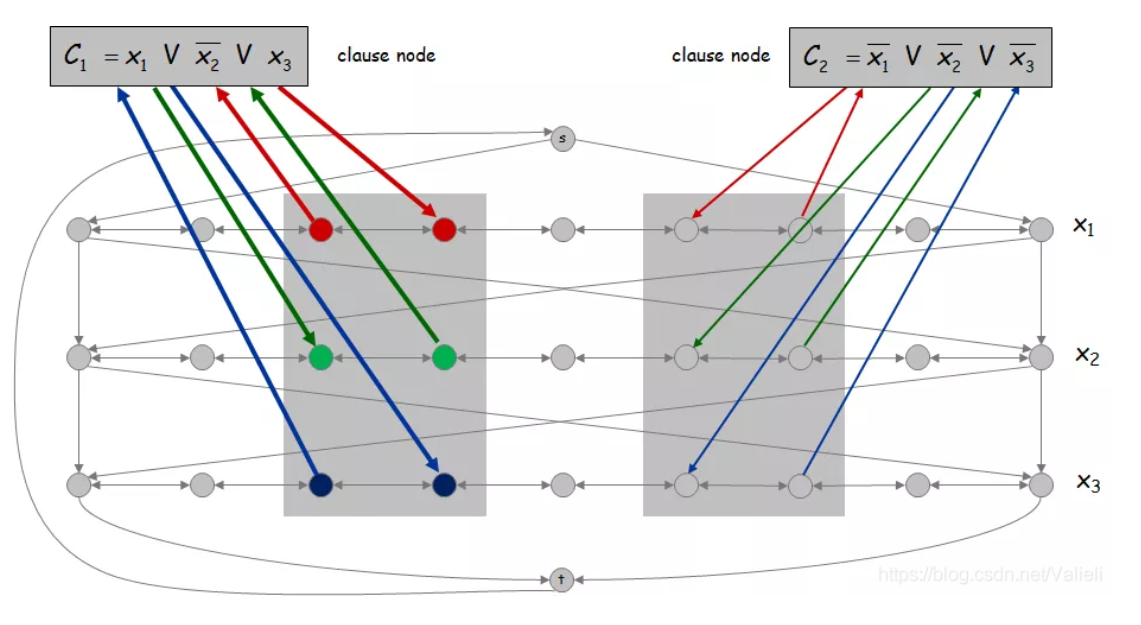
\includegraphics[scale=0.6]{./figure/8.5.2.png}
		\caption{$3SAT$~to~$HAMPATH$}
		\label{F080502}
   \end{figure} 

	\colorbox{green}{定理8.36} $UHAMPATH$(无向图的哈密顿回路)是$NP$完全的。
	
	\textbf{证明思路} \quad 从$HAMPATH$归约到$UHAMPATH$。有向图的一个点$u$,拆成无向图的三个点$u^{in},u^{mid},u^{out}$。

\subsubsection{子集和问题}
	
	\colorbox{green}{定理8.34} $SUBSET-SUM$是$NP$完全的,示意图 \ref{F080503}。
	
	\textbf{证明思路} \quad 从$3SAT$归约到$SUBSET-SUM$

	\begin{figure}[htb]
		\centering
		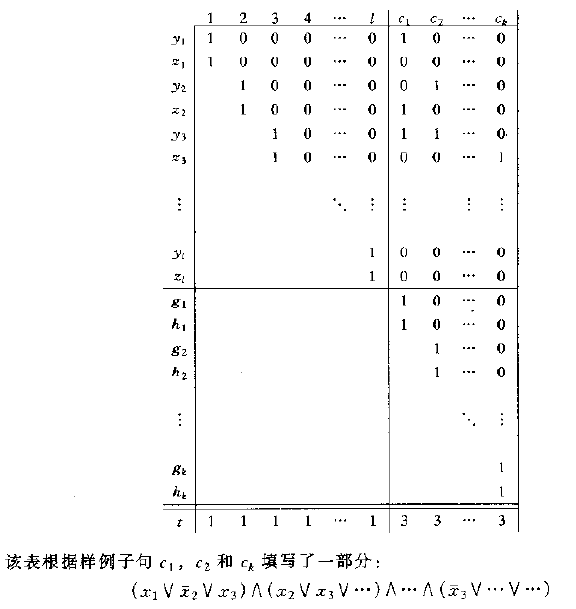
\includegraphics[scale=0.6]{./figure/8.5.3.png}
		\caption{$3SAT$~to~$SUBSET-SUM$}
		\label{F080503}
   \end{figure} 
   
\subsubsection{补充}

	\colorbox{green}{补充定理} 最小旅行商问题$TSP$是$NP$完全的。
	
	\textbf{证明思路} \quad 从哈密顿回路问题归约到$TSP$问题,每条路径的长度都为$1$。
	
	\colorbox{green}{补充定理} $k-\text{独立集}$是$NP$完全的。
	
	\textbf{证明思路} \quad 从$k-CLIQUE$归约到$k-\text{独立集}$。

	更多NP完全问题的归约关系图 \ref{F080504}
	\begin{figure}[htb]
		\centering
		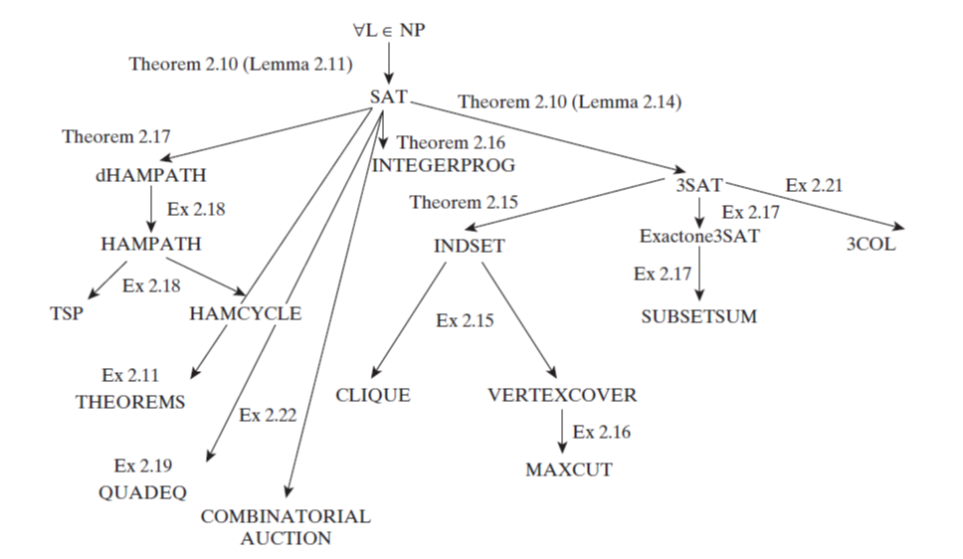
\includegraphics[scale=0.6]{./figure/8.5.4.png}
		\caption{More NP Problems}
		\label{F080504}
   \end{figure} 

	
	
\section{空间复杂性}

	\colorbox{yellow}{定义9.1} 空间复杂度:$O(f(n))$。其中,$f: \mathcal{N} \rightarrow \mathcal{N}$。

	\colorbox{yellow}{定义9.2} 空间复杂性类:$SPACE(f(n))$和$NSPACE(f(n))$。前者指确定型图灵机,后者指非确定型图灵机。
	
	\colorbox{pink}{例9.3} $SAT$问题可以在线性空间内运行。
	
	\colorbox{pink}{例9.4} 对于问题
		$$ALL_{NFA}=\{<A>|A~is~NFA~and~L(A)=\Sigma^*\}$$

		该问题在非确定的空间$O(n)$内运行。
	
\subsection{萨维奇定理}

	\colorbox{green}{定理9.5} 萨维奇定理

		对于任何函数:$f: \mathcal{N} \rightarrow \mathcal{N}$,其中$f(n)\geq n$,
			$$NSPACE(f(n))\subseteq SPACE(f(n)^2)$$

		\textbf{证明思路}\quad 使用分治的方式,总空间复杂度为$O(\log{|\Sigma|^{f(n)}} \times f(n))=O(f(n)^2)$。

\subsection{$PSPACE$类}
	\colorbox{yellow}{定义9.6} $PSPACE$是在确定型图灵机上、在多项式\textbf{空间}内可判定的语言类。换言之,
		$$PSPACE=\cup_{k}{SPACE(n^k)}$$
	
	同理,可以定义$NPSPACE$。
	
	需要注意的是,\textbf{$PSPACE$对于一个语言的补集是封闭的},由于空间有上限,所以格局有上限(设为$q$),计算次数超过$2^q$即出现循环,可以判定此时不会停机。
	
	通过\textbf{萨维奇定理},可以推到得到$NPSPACE=PSPACE$。
	
	总结所定义的复杂性类之间的关系:
	$$ P\subseteq NP \subseteq PSPACE = NPSPACE \subseteq EXPTIME $$

\subsection{$PSPACE$完全性}
	\colorbox{yellow}{定义9.7} 语言$B$是$PSPACE$完全的,若它满足两个条件:
	
	\qquad \textbf{1)} $B$属于$PSPACE$。

	\qquad \textbf{2)} $PSPACE$中的每一个语言$A$多项式时间可归约到$B$。
	
	若只满足条件2,则称它为\textbf{$PSPACE$难的}。

\subsubsection{问题$TQBF$}

	TQBF问题就是要判定一个全量词化的布尔公式是真还是假。定义语言
	$$TQBF=\{<\phi>|\phi~is~a~true~fully~quantified~Boolean~formula\}$$
	
	\colorbox{green}{定理9.8} $TQBF$是$PSPACE$完全的
	
	\textbf{证明思路}
		
		\qquad 条件1:构造算法,说明空间复杂度为多项式的。
		
		\qquad 条件2:利用分治的思想,将一个问题拆成两部分,使用$\exists$(存在一种拆法)和$\forall$(对于所有的递归步骤)两种量词进行构造:
		$$\phi_{c_1,c_2,t}=\exists m_1 \forall (c_3,c_4)\in \{(c_1,m1), (m_1,c_2\}[\phi_{c_3,c_4,\lceil \frac{t}{2}\rceil}]$$
		
		
\subsubsection{博弈的必胜策略}

	公式博弈游戏:玩家按照顺序给$x_1,\dots,x_n$赋值。最后公式真值为TRUE则玩家E胜利,否则玩家A胜利。

	\colorbox{pink}{例9.9} 公式博弈:$\exists x_1 \forall x_2 \exists x_3[(x_1 \vee x_2) \land (x_2 \vee x_3) \land (\overline{x_2} \vee \overline{x_3})]$

	公式博弈的语言如下所示:
	\begin{multline}
		FORMULA-GAME=\{<\phi>|Player~E~has~a~winning~strategy \\
		in~the~formula~game~associated~with~\phi\}
	\end{multline}

	\colorbox{green}{定理9.10} $FORMULA-GAME$是$PSPACE$完全的
	
	\textbf{证明思路} \quad 由于公式中存在$\exists$和$\forall$量词,所以$FORMULA-GAME=TQBF$。

\subsubsection{广义地理学}

	广义地理学游戏:对于一个图,玩家轮流在图的结点上填写地理名词,对于有向边$A \rightarrow B$,要求$B$以$A$的结尾字母开头。

	广义地理学的语言如下所示:
	\begin{multline}
		GG=\{<G,b>|Player~I~has~a~winning~strategy \\
		for~the~generalized~geography~game~played~on~graph~G~starting~at~node~b\}
	\end{multline}

	\colorbox{green}{定理9.11} $GG$是$PSPACE$完全的

	\textbf{证明思路}
		
		\qquad 条件1:构造算法,说明空间复杂度为多项式的。
		
		\qquad 条件2: 将$FORMULA-GAME$转化为$GG$,示意图\ref{F0911}。玩家E想使公式为真,玩家A想使公式为假。最后一个钻石是E来选择,那么A走完这个钻石,E走到结点$c$上。此时,如果想要公式成假,那么只要有一个子式为假即可,即这个子式中的任意一个结点之前都没走过。那么E和A再各走一步之后,E无路可走,此时原式为假,A获胜。否则,E走那条连接之前走过的结点的边,A无路可走,此时原式为真,E获胜。

		\begin{figure}[htb]
			\centering
			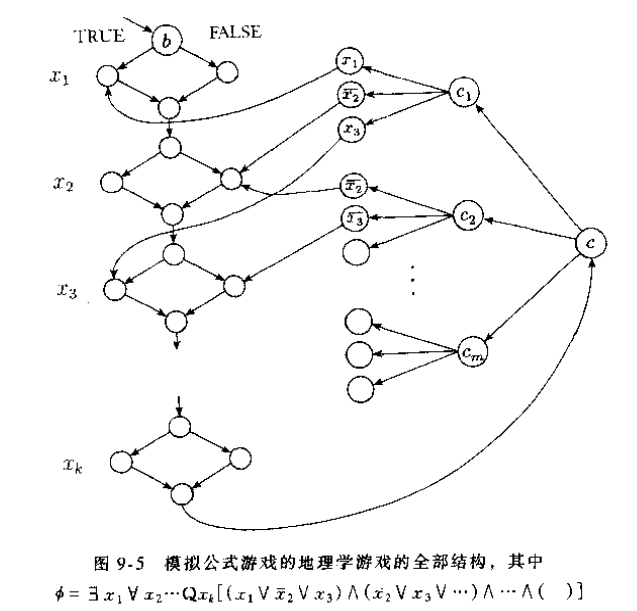
\includegraphics[scale=0.8]{./figure/9.11.png}
			\caption{$FORMULA-GAME$~to~$GG$}
			\label{F0911}
    	\end{figure} 

\subsection{$L$类和$NL$类}

	\colorbox{yellow}{定义9.12} $L$和$NL$
	
		\qquad $L$是确定型图灵机在对数空间内可判定的语言类,即$L=SPACE(\log{n})$。
		
		\qquad $NL$是确定型图灵机在对数空间内可判定的语言类,即$L=NSPACE(\log{n})$。
		
	需要注意的是,在亚线性空间界限下,图灵机有两条纸带,一条只读,一条可写,模仿内存和外存。

	\colorbox{pink}{例9.13} 语言$A=\{0^k1^k|k\geq 0\}$是$L$的成员。

	\colorbox{pink}{例9.14} 语言$PATH=\{<G,s,t>|G~is~a~directed~graph~that~has~a~directed~path~from~s~to~t\}$是$NL$的成员

	\colorbox{yellow}{定义9.15} 若$M$是一个有单独的只读输入带的图灵机,$\omega$是输入,则\textbf{$M$在$\omega$上的格局}是状态、工作带和两个读写头位置的一种设置。输入$\omega$不最为$M$在$\omega$上的格局的一部分。

\subsection{$NL$完全性}

	\colorbox{yellow}{定义9.16} 
	
		\qquad \textbf{对数空间转换器}是有一条只读输入带、一条只写输出带和一条读写工作带的图灵机。

		\qquad \textbf{对数空间可计算函数}:$f:\Sigma^* \rightarrow \Sigma^*$
		
		\qquad 如果语言$A$通过对数空间可计算函数$f$映射可规约到语言$B$,则称\textbf{$A$对数空间可规约到$B$},记为$A\leq_L B$。
		
	\colorbox{yellow}{定义9.17} 语言$B$是\textbf{$NL$完全的},如果
	
		\qquad 1)$B \in NL$,并且
		
		\qquad 2)$NL$中的每个$A$对数空间可规约到$B$。

	\colorbox{green}{定理9.18} 若$A\leq_L B$且$B\in L$,则$A\in L$。

	\colorbox{gray}{推论9.19} 若有一个$NL$完全语言属于$L$,则$L=NL$。

	\colorbox{green}{定理9.20} $PATH$是$NL$完全的。
	
	\textbf{证明思路} \quad 把字符串$\omega$映射成一个图,图中结点对应的是$NTM$在输入$\omega$上的格局。

	\colorbox{gray}{推论9.21} $NL\subseteq P$
	
	\textbf{证明思路} \quad 一个结论:消耗空间为$O(f(n))$的图灵机在$n2^{O(f(n))}$下运行。

\subsection{$NL$等于$coNL$}

	$L\in coNL$ 当且仅当 $\overline{L} \in NL$

	\colorbox{green}{定理9.22} $NL=coNL$

	\textbf{证明思路} \quad 证明$\overline{PATH} \in NL$。由于$PATH$是$NL$完全的,所以当语言$A$可以归约到$PATH$,那么$\overline{A}$可以归约到$\overline{PATH}$,因此$A \in coNL$,即可证明$NL=coNL$。
	
	当前已知的几个复杂性类之间相互关系的认识总结如下:
	$$ L \subseteq NL = coNL \subseteq P \subseteq PSPACE $$

\end{document}